\chapter{RNA-Seq 数据分布的不均匀性}
\label{chap-rna-seq-nonunif}

\section{介绍}
根据 \ref{len-est-real-rna-seq} 中对于实际 RNA-Seq 数据的分析, 
我们发现 RNA-Seq 数据并不符合理想的均匀分布 (图 \ref{rna-seq-bias}). 
\onlinecite{oshlack2009transcript}, \onlinecite{roberts2011improving}, 
\onlinecite{20132535}, \onlinecite{21176179}, \onlinecite{20167110}, 和
\onlinecite{li2010rna} 等也均对 RNA-Seq 实验数据分布的不均匀性进行了研究和讨论. 

\begin{figure}[!t]
\centering
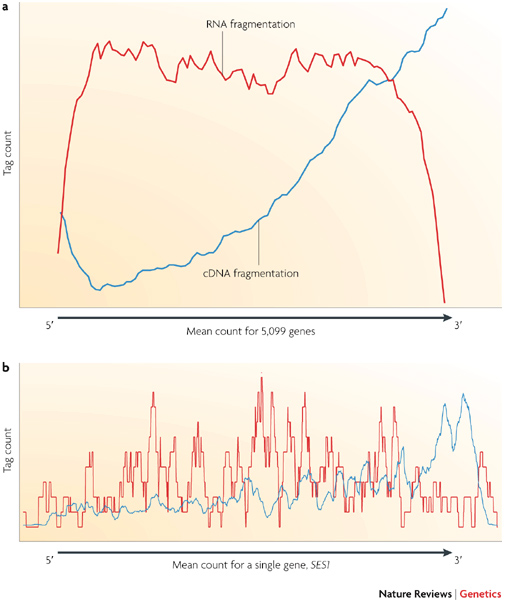
\includegraphics[width=\textwidth]{figures/nonunif/rna-seq-bias.jpg}
\caption{实际 RNA-Seq 数据中读段的位置分布 \cite{wang2009rna}}
\label{rna-seq-bias}
\end{figure}

\section{数据分析}
我们对来自 ENCODE \cite{encode} 的 RNA-Seq 数据 
\footnote{\url{http://hgdownload.cse.ucsc.edu/goldenPath/hg19/encodeDCC/wgEncodeCaltechRnaSeq/wgEncodeCaltechRnaSeqGm12878R1x75dAlignsRep2V2.bam}} 
进行了分析, 试图发现 RNA-Seq 数据读段分布的一些规律. 

\subsection{方法}
\subsubsection{检验均匀分布的 p-value 的计算}
给定一个转录本, 在计算检验均匀分布的 p-value 时, 
我们将转录本划分成若干段, 在统计出每一段中的读段起始书目后, 使用 $\chi^2$ 统计量, 
通过 parametric bootrstrap \cite{efron1993introduction} 计算 p-value. 

\subsection{结果}


